\documentclass[conference]{IEEEtran}
\IEEEoverridecommandlockouts
% The preceding line is only needed to identify funding in the first footnote. If that is unneeded, please comment it out.
\usepackage{cite}
\usepackage{amsmath,amssymb,amsfonts}
\usepackage{algorithmic}
\usepackage{graphicx}
\usepackage{textcomp}
\usepackage{xcolor}
\usepackage{listings}
\usepackage{acronym}
\usepackage{listing-style}
\usepackage{subcaption}
\usepackage{tikz}
\usetikzlibrary{arrows,shapes.geometric,positioning,automata,calc}
\usepackage[hidelinks]{hyperref}
\usepackage[inline]{enumitem}

\acrodef{dsl}[DSL]{domain-specific language}
\acrodef{iot}[IoT]{Internet of Things}
\acrodef{cas}[CAS]{collective adaptive system}
\acrodef{qos}[QoS]{quality of service}

\usepackage{cleveref}

\def\BibTeX{{\rm B\kern-.05em{\sc i\kern-.025em b}\kern-.08em
    T\kern-.1667em\lower.7ex\hbox{E}\kern-.125emX}}
    
\newcommand{\meta}[1]{{\color{blue}#1}}   

\lstset{xleftmargin=0.3cm,numbersep=5pt} 

\makeatletter
\newcommand{\linebreakand}{%
  \end{@IEEEauthorhalign}
  \hfill\mbox{}\par
  \mbox{}\hfill\begin{@IEEEauthorhalign}
}
\makeatother

    
\begin{document}

\title{Declarative Deployment Reconfiguration of Pulverised Collective Adaptive Systems at Runtime
\thanks{
    This work has been supported by the Italian PRIN Project COMMON-WEARS (2020HCWWLP) and the EU/MUR FSE REACT-EU PON R\&I 2014-2020.
}
}

\author{\IEEEauthorblockN{1\textsuperscript{st} Danilo Pianini}
\IEEEauthorblockA{\textit{Department of Computer Science and Engineering} \\
\textit{Alma Mater Studiorum---Università di Bologna}\\
Cesena, Italy \\
danilo.pianini@unibo.it}
\and
\IEEEauthorblockN{2\textsuperscript{nd} Roberto Casadei}
\IEEEauthorblockA{\textit{Department of Computer Science and Engineering} \\
\textit{Alma Mater Studiorum---Università di Bologna}\\
Cesena, Italy \\
roby.casadei@unibo.it}
\linebreakand
\IEEEauthorblockN{3\textsuperscript{rd} Nicolas Farabegoli}
\IEEEauthorblockA{\textit{Department of Computer Science and Engineering} \\
\textit{Alma Mater Studiorum---Università di Bologna}\\
Cesena, Italy \\
nicolas.farabegoli@unibo.it}
\and
\IEEEauthorblockN{4\textsuperscript{th} Mirko Viroli}
\IEEEauthorblockA{\textit{Department of Computer Science and Engineering} \\
\textit{Alma Mater Studiorum---Università di Bologna}\\
Cesena, Italy \\
mirko.viroli@unibo.it}
}

\maketitle

\begin{abstract}
In recent years,
the infrastructure supporting the execution of situated distributed computations
evolved with a fast pace.
%
Modern collective adaptive applications -- as found in the Internet of Things, swarm robotics, and social computing -- are designed to be executed on very diverse devices
and to be deployed on infrastructures composed of devices ranging from cloud servers to wearable devices,
constituting together a cloud-edge continuum.
%
The availability of such an infrastructure opens to better resource utilisation and performance,
but, contextually, introduces new challenges to software designers,
as applications must be conceived to be able to adapt their deployment to changing deployment domains and conditions.
%
In this paper,
we introduce a practical framework for the development of collective adaptive systems
based on the concept of \emph{pulverisation},
meant to neatly separate business logic and deployment concerns,
allowing applications to be defined independent of the infrastructure they will execute upon.
%
The framework is based on a domain-specific language capturing,
in a declarative fashion,
pulverised application components, device capabilities, resource allocation, and (runtime re-) configuration policies.
%
The framework, implemented in Kotlin multiplatform and available as open source,
is then evaluated in a small-scale real-world demo and in a city-scale simulated scenario,
 \meta{showing that ???}.
\end{abstract}

\begin{IEEEkeywords}
runtime reconfiguration, distributed systems, self-adaptation, self-organisation, pulverisation, deployment.
\end{IEEEkeywords}

\newcommand{\ourframework}{\textsc{pulse-refrakt}}

%\meta{LIMIT 10 pages incl. refs; DEADLINE 19 may}

\section{Introduction}\label{sec:introduction}

Recent technological and scientific advances
 are extending 
 both the \emph{kinds of applications and systems} that are being addressed  
 as well as their \emph{supporting infrastructure}~\cite{DBLP:journals/iot/GillXOPBSGSWASM22}.
%
Emerging applications
 are, for instance, those based on \emph{\acp{cas}}~\cite{DBLP:journals/computer/Abowd16,DBLP:journals/sttt/NicolaJW20},
 namely collections of devices and agents
 that interact to solve problems or provide services while adapting \emph{as a whole} to dynamic environments.
%
Examples include 
  \ac{iot} deployments, 
  swarms of robots,
  social computing systems,
  crowds of wearable-augmented people, and so on---supporting activities like monitoring,
  transportation, coordination, and other forms of collective intelligence~\cite{casadei2023artl-ci}.
%
Regarding infrastructure,
 it is mounting the idea of the \emph{cloud-edge continuum}~\cite{DBLP:journals/iot/BittencourtISFM18}: 
a multi-layer heterogeneous network of devices (ranging from large and powerful cloud servers to small connected \emph{things})
on which software can compute, store, and exchange data in a distributed fashion, while 
optimising for performance and resource utilisation.
%

This kind of infrastructure is also valuable for  \acp{cas}~\cite{DBLP:journals/tpds/HongCHGZ19,DBLP:journals/comsur/WangZZMLW20,DBLP:journals/comsur/AfrinJRRWH21,IEEE-IoTJ-pulverization-simulation},
which generally feature components that,
depending on the conditions at hand,
could benefit from being deployed on different devices or from \emph{offloading} some of their  tasks.
%
However, exploiting this infrastructure,
 poses new challenges to \ac{cas} application designers.
%
Commonly, in fact, applications are designed with a specific infrastructure in mind,
whose assumptions unavoidably leak into the application logic~\cite{Spolsky2004},
unless captured and encapsulated away from it:
the higher the coupling between the application and the infrastructure,
the harder it is for the former to exploit the latter's full potential and adapt to changes.

The general solution is to devise 
 a reasonable partitioning of the software system
 and a corresponding (dynamic) deployment plan 
 defining the mapping between the software components and the target deployment domain~\cite{DBLP:journals/jss/ArcangeliBL15}.
%
In the context of \acp{cas},
 previous work proposes an application partitioning schema,
 called \emph{pulverisation}~\cite{FI2020-pulverization},
 the fosters the decoupling of business logic and deployment concerns.
%
In short, the core idea is to consider devices as \emph{logical} entities,
whose software can be designed as (or broken down to, if already existing) an ensemble of \emph{five components
(behaviour, state, communication, sensors, and actuators)}
 that can be deployed with flexibility on available infrastructure without (ideally) affecting application functionality. %whose actual host can be decided at deployment time.
%
This way, the designer can focus on the business logic at hand,
delaying an optimised deployment to later stages of the sofware design,
thus gaining resilience to changes in the infrastructure or in non-functional requirements.
%
One limitation of previous work on pulverisation regards dynamicity:
although the application can be deployed on arbitrary systems,
there is no support for the reconfiguration of components at runtime, as a reaction to changing conditions or requirements.

In this work,
we continue the research on pulverised systems by providing two key contributions:
\textbf{first}, we extend the theoretical framework of pulverisation by adding support for
\emph{runtime configuration rules}, allowing pulverised components to move at runtime across different hosts;
\textbf{second}, we provide a practical implementation in Kotlin called \ourframework{} which,
to the best of our knowledge,
is the first \emph{practical framework supporting pulverisation}. % for a general-purpose language.
%
To evaluate \ourframework{}, we exercise it through two case studies:
a small-scale real-wold demonstration, and a city-scale simulated scenario.

%\meta{
%\begin{itemize}
%    \item need for deployment-independent specs
%    \item need for runtime reconfiguration (achieve \ac{qos} in face of changing conditions --- green computing?)
%    \item declarativity over imperative approaches (note: can be compared with the trend in general softeng/build systems)
%\end{itemize}
%}

The manuscript is organised as follows.
%
\Cref{sec:background} provides background on deployment and pulverisation.
%
\Cref{sec:contribution} describes the proposed \ac{dsl} and platform.
%
\Cref{sec:evaluation} provides an evaluation of the approach.
%
\Cref{sec:rw} covers related work.
%
Finally, \Cref{sec:conclusion} concludes the paper and highlights directions for future work.

\section{Background}\label{sec:background}

\subsection{Deployment and Reconfiguration: Basic Concepts}\label{sec:background:dep}

The \emph{deployment view} is a well-known architectural viewpoint for software systems,
concerned with the mapping of \emph{software components} to \emph{physical machines}~\cite{DBLP:journals/software/Kruchten95}, 
 and supported by modelling notations like \emph{UML Deployment diagrams}.
%
Here, we provide a brief introduction to deployment and reconfiguration, based on the conceptual characterisation of~\cite{DBLP:journals/jss/ArcangeliBL15,carzaniga1998characterization}.
%
A \emph{site} is a set of computers (\emph{hosts}) that may host a \emph{software system}, i.e., a coherent collection of artifacts.
%
\emph{(Software) Deployment} is the process of moving and making a software system available and operational from one or more \emph{producer sites} to a target set of \emph{consumer sites}, also called the \emph{deployment domain}.
%
The \emph{deployment plan} defines 
 the mapping between the software system
 and the deployment domain,
 possibly augmented with further information (e.g., metadata, constraints, preferences).
%
Common deployment-related activities 
 include: (i) \emph{release/update} of the software system at the producer site;
 (ii) \emph{installation/deinstallation} at/from the consumer sites;
 (iii) \emph{activation/deactivation}, for starting/stopping the components;
 (iv) \emph{reorganisation} of the software system;
 and (v) \emph{redistribution}, i.e., changing the deployment plan.
%
According to the analytical framework of~\cite{DBLP:journals/jss/ArcangeliBL15},
  the problem of (automatic) deployment of distributed software system can be addressed by considering
 (i) the nature of the software to be deployed (e.g., how the software system is split into components);
 (ii) the nature of the deployment domain (i.e. the characteristics and topology of the available infrastructure);
 (iii) how the deployment is designed (e.g., how the deployment plan is specified);
 and 
 (iv) how the deployment is performed (e.g., how deployment activities are carried out).
%
By an operational point of view, 
 deployment may be supported by a \emph{middleware}~\cite{DBLP:journals/cacm/GazisK22}.
%
Related work covering these issues is provided in \Cref{sec:rw}.
%
In the following, we introduce the deployment approach 
  that we extend and upon which we develop \ourframework{}.



\begin{figure}
\tikzset{-,
  host/.style={rectangle,draw,line width={2pt},inner sep=10pt,
  	outer sep=0, minimum height=1.5cm, minimum width=1.8cm, %text height=0.2cm, 
  	text depth=0.5cm,
  	fill=black!10!white
  },
  node/.style={rectangle,draw,dotted,line width={1pt}, inner sep=2pt, 
  	fill=blue!20!white,
  	font=\large
  },
  nodeA/.style={node,fill=red!20!white},
  nodeB/.style={node,fill=green!20!white},
  nodeC/.style={node,fill=black!30!white},
  nodeD/.style={node,fill=white!20!white},
  plink/.style={line width=2pt},
  llink/.style={dotted,line width=2pt,red},
  hostThin/.style={rectangle,draw,line width={0.5pt},inner sep=10pt,
  	outer sep=0, minimum height=1.1cm, minimum width=1.8cm, %text height=0.2cm, 
  	text depth=0.5cm,
  	fill=black!10!white
  },
  lnode/.style={node,minimum width=0.55cm,minimum height=0.55cm},
  loglink/.style={->,line width=1.5pt}
}
\def\nm{0.35cm} %nm = node margin offset
\def\tpscale{0.7}
\newcommand{\agent}{device}
\newcommand{\LSens}{\boldsymbol{\sigma}}
\newcommand{\LComp}{\boldsymbol{\beta}}
\newcommand{\LComm}{\boldsymbol{\chi}}
\newcommand{\LAct}{\boldsymbol{\alpha}}
\newcommand{\LState}{\boldsymbol{\kappa}}

\begin{minipage}{\columnwidth}
\centering
\begin{tikzpicture}[every node/.style={scale=1}]
\node[hostThin,minimum width=3.4cm,minimum height=3cm,dashed]
 (h1) [label={[yshift=0.35cm]above:{\textbf{logical \agent{}}}}] {};

\node[lnode] (d1) at (h1.north west) [xshift=\nm,yshift=-\nm,label=above:{behaviour}] {$\LComp$};
\node[lnode] (d2) at (h1.north east) [xshift=-\nm,yshift=-\nm,label=above:{communication}] {$\LComm$};
\node[lnode] (d3) at (h1.center) [xshift=0,yshift=0,label=right:{state/knowledge}] {$\LState$};
\node[lnode] (d4) at (h1.south west) [xshift=\nm,yshift=\nm,label=below:{sensors}] {$\LSens$};
\node[lnode] (d5) at (h1.south east) [xshift=-\nm,yshift=\nm,label=below:{actuators}] {$\LAct$};

\node[hostThin,minimum width=2.3cm,minimum height=2.3cm,dashed]
 (h2) [right=2cm of h1, label={above:{\textbf{neighbour \agent{}}}}] {};

\node[lnode] (d21) at (h2.north west) [xshift=\nm,yshift=-\nm] {$\LComm$};
\node[lnode] (d22) at (h2.north east) [xshift=-\nm,yshift=-\nm] {$\LComp$};
\node[lnode] (d23) at (h2.center) [xshift=0,yshift=0] {$\LState$};
\node[lnode] (d24) at (h2.south west) [xshift=\nm,yshift=\nm] {$\LSens$};
\node[lnode] (d25) at (h2.south east) [xshift=-\nm,yshift=\nm] {$\LAct$};

\draw[loglink] (d1) -- (d3);
\draw[loglink] (d2) -- (d3);
\draw[loglink] (d3) -- (d1);
\draw[loglink] (d3) -- (d2);
\draw[loglink] (d4) -- (d3);
\draw[loglink] (d3) -- (d5);

\draw[loglink] (d21) -- (d23);
\draw[loglink] (d22) -- (d23);
\draw[loglink] (d23) -- (d21);
\draw[loglink] (d23) -- (d22);
\draw[loglink] (d24) -- (d23);
\draw[loglink] (d23) -- (d25);

\draw[loglink] (d2.east) -- (d21.west);
\draw[loglink] (d21.west) -- (d2.east);


\end{tikzpicture}
\subcaption{A logical device, split into sub-components, and one of its neighbours.\label{fig:pulv:dev}}
\end{minipage}
\\[0.2cm]
\begin{minipage}{\columnwidth}
\def\nm{0.3cm} %nm = node margin offset

\begin{minipage}{0.48\columnwidth}\centering
\begin{tikzpicture}[node distance=1.0cm and 0.5cm,every node/.style={scale=\tpscale}]
% physical nodes
\node[host] (h1) [anchor=north,label=above:{}] {};
\node[host] (h2) [right=of h1,label=above:{}] {};
\node[host] (h3) [below=of h1, label=above:{}] {};
\node[host] (h4) [right=of h3, label=above:{}] {};

\node[node] (n11) at (h1.south west) [xshift=\nm,yshift=\nm] {$\LSens$};
\node[node] (n12) at (h1.south east) [xshift=-\nm,yshift=\nm] {$\LComm$};
\node[node] (n13) at (h1.north east) [xshift=-\nm,yshift=-\nm] {$\LAct$};
\node[node] (n14) at (h1.north west) [xshift=\nm,yshift=-\nm] {$\LComp$};
\node[node] (n15) at (h1) [] {$\LState$};
% logical node 2
\node[nodeA] (n21) at (h2.south west) [xshift=\nm,yshift=\nm] {$\LComm$};
\node[nodeA] (n22) at (h2.south east) [xshift=-\nm,yshift=\nm] {$\LAct$};
\node[nodeA] (n23) at (h2.north east) [xshift=-\nm,yshift=-\nm] {$\LSens$};
\node[nodeA] (n24) at (h2.north west) [xshift=\nm,yshift=-\nm] {$\LComp$};
\node[nodeA] (n25) at (h2) [] {$\LState$};
% logical node 3
\node[nodeB] (n31) at (h3.south west) [xshift=\nm,yshift=\nm] {$\LSens$};
\node[nodeB] (n32) at (h3.south east) [xshift=-\nm,yshift=\nm] {$\LAct$};
\node[nodeB] (n33) at (h3.north east) [xshift=-\nm,yshift=-\nm] {$\LComm$};
\node[nodeB] (n34) at (h3.north west) [xshift=\nm,yshift=-\nm] {$\LComp$};
\node[nodeB] (n35) at (h3) [] {$\LState$};
% logical node 4
\node[nodeC] (n41) at (h4.south west) [xshift=\nm,yshift=\nm] {$\LSens$};
\node[nodeC] (n42) at (h4.south east) [xshift=-\nm,yshift=\nm] {$\LAct$};
\node[nodeC] (n43) at (h4.north east) [xshift=-\nm,yshift=-\nm] {$\LComp$};
\node[nodeC] (n44) at (h4.north west) [xshift=\nm,yshift=-\nm] {$\LComm$};
\node[nodeC] (n45) at (h4) [] {$\LState$};

% physical links
\draw[plink] 
	(h1) -- (h2)
	(h2) -- (h3)
	(h2) -- (h4)
	(h3) -- (h4)
;
% logical links
\draw[llink]
    (n12) to [] (n21)
    (n21) to [] (n44)
    (n21) to [bend right=30] (n33)
    (n33) to [] (n44);
\end{tikzpicture}
\subcaption{Peer-to-peer architecture: one-to-one mapping between logical and physical devices, with no offloading.\label{fig:pulv:p2p}}
\end{minipage}
%\hfill
%\begin{minipage}{0.48\columnwidth}\centering
%\begin{tikzpicture}[node distance=1.0cm and 0.5cm,
%every node/.style={scale=\tpscale}]
%
%% physical nodes
%\node[host,minimum width=1.5cm] (h1) [anchor=north,label=above:{}] {};
%\node[host,minimum width=1.5cm] (h2) [right=of h1,label=above:{}] {};
%\node[host,minimum width=1.5cm] (h3) [right=of h2, label=above:{}] {};
%\node[host,minimum width=2.5cm] (he) [above right=0.6cm and -1cm of h1,label=above:{}] {};
%\node[host,minimum width=3.5cm] (h5) [above=2.6cm of h2,label=right:{}] {};
%
%\node[node] (n11) at (h1.south west) [xshift=\nm,yshift=\nm] {$\LSens$};
%\node[node] (n12) at (h1.south east) [xshift=-\nm,yshift=\nm] {$\LAct$};
%\node[node] (n13) at (h1.north east) [xshift=-\nm,yshift=-\nm] {$\LState$};
%\node[node] (n14) at (h1.north west) [xshift=\nm,yshift=-\nm] {$\LComp$};
%\node[node] (n15) at (he) [xshift=-2*\nm] {$\LComm$};
%% logical node 2
%\node[nodeA] (n21) at (h2.south west) [xshift=\nm,yshift=\nm] {$\LSens$};
%\node[nodeA] (n22) at (h2.south east) [xshift=-\nm,yshift=\nm] {$\LAct$};
%\node[nodeA] (n23) at (h2.north east) [xshift=-\nm,yshift=-\nm] {$\LState$};
%\node[nodeA] (n24) at (h2.north west) [xshift=\nm,yshift=-\nm] {$\LComp$};
%\node[nodeA] (n25) at (he) [xshift=0] {$\LComm$};
%% logical node 3
%\node[nodeB] (n31) at (h3.south west) [xshift=\nm,yshift=\nm] {$\LSens$};
%\node[nodeB] (n32) at (h3.south east) [xshift=-\nm,yshift=\nm] {$\LAct$};
%\node[nodeB] (n33) at (h3.north east) [xshift=-\nm,yshift=-\nm] {$\LState$};
%\node[nodeB] (n34) at (h3.north west) [xshift=\nm,yshift=-\nm] {$\LComp$};
%\node[nodeB] (n35) at (h5) [xshift=2*\nm] {$\LComm$};
%
%% physical links
%\draw[plink] 
%	(h1) -- (he)
%	(h2) -- (he)
%	(h3) -- (h5)
%	(he) -- (h5);
%
%\draw[llink]
%    %(n15) to [bend left=20] (n35)
%    (n25) to [bend left=30] (n35);
%\end{tikzpicture}
%\subcaption{Communication component offloaded.\label{fig:pulv:comm}}
%\end{minipage}
%\\[0.2cm]
%\begin{minipage}{0.48\columnwidth}\centering
%\begin{tikzpicture}[node distance=1.0cm and 0.5cm,
%every node/.style={scale=\tpscale}]
%
%% physical nodes
%\node[host,minimum width=1.5cm] (h1) [anchor=north,label=above:{}] {};
%\node[host,minimum width=1.5cm] (h2) [right=of h1,label=above:{}] {};
%\node[host,minimum width=1.5cm] (h3) [right=of h2, label=above:{}] {};
%\node[host,minimum width=2.5cm] (he) [above right=0.6cm and -1cm of h1,label=above:{}] {};
%\node[host,minimum width=3.5cm] (h5) [above=2.6cm of h2,label=right:{}] {};
%
%\node[node] (n11) at (h1.south west) [xshift=\nm,yshift=\nm] {$\LSens$};
%\node[node] (n12) at (h1.south east) [xshift=-\nm,yshift=\nm] {$\LAct$};
%\node[node] (n13) at (he.north) [xshift=-2*\nm,yshift=-\nm] {$\LComm$};
%\node[node] (n14) at (h1.north) [yshift=-\nm] {$\LComp$};
%\node[node] (n15) at (he.south) [xshift=-2*\nm,yshift=\nm] {$\LState$};
%% logical node 2
%\node[nodeA] (n21) at (h2.south west) [xshift=\nm,yshift=\nm] {$\LSens$};
%\node[nodeA] (n22) at (h2.south east) [xshift=-\nm,yshift=\nm] {$\LAct$};
%\node[nodeA] (n23) at (he.north) [xshift=0*\nm,yshift=-\nm] {$\LComm$};
%\node[nodeA] (n24) at (h2.north) [yshift=-\nm] {$\LComp$};
%\node[nodeA] (n25) at (he.south) [xshift=0,yshift=\nm] {$\LState$};
%% logical node 3
%\node[nodeB] (n31) at (h3.south west) [xshift=\nm,yshift=\nm] {$\LSens$};
%\node[nodeB] (n32) at (h3.south east) [xshift=-\nm,yshift=\nm] {$\LAct$};
%\node[nodeB] (n33) at (h5.south) [xshift=2*\nm,yshift=\nm] {$\LComm$};
%\node[nodeB] (n34) at (h3.north) [yshift=-\nm] {$\LComp$};
%\node[nodeB] (n35) at (h5.south) [xshift=4*\nm,yshift=\nm] {$\LState$};
%
%% physical links
%\draw[plink] 
%	(h1) -- (he)
%	(h2) -- (he)
%	(h3) -- (h5)
%	(he) -- (h5);
%
%\draw[llink]
%    %(n15) to [bend left=20] (n35)
%    (n23) to [bend left=20] (n33);
%\end{tikzpicture}
%\subcaption{Communication and state components offloaded.\label{fig:pulv:state}}
%\end{minipage}
\hfill
\begin{minipage}{0.48\columnwidth}
\begin{tikzpicture}[node distance=1.0cm and 0.5cm,
every node/.style={scale=\tpscale}]

% physical nodes
\node[hostThin,minimum width=1.5cm] (h1) [anchor=north,label=above:{}] {};
\node[hostThin,minimum width=1.5cm] (h2) [right=of h1,label=above:{}] {};
\node[hostThin,minimum width=1.5cm] (h3) [right=of h2, label=above:{}] {};
\node[host,minimum width=2.5cm] (he) [above right=0.6cm and -1cm of h1,label=above:{}] {};
\node[host,minimum width=3.5cm] (h5) [above=2.6cm of h2,label=right:{}] {};

\node[node] (n11) at (h1.south west) [xshift=\nm,yshift=\nm] {$\LSens$};
\node[node] (n12) at (h1.south east) [xshift=-\nm,yshift=\nm] {$\LAct$};
\node[node] (n13) at (he.south east) [xshift=-4*\nm,yshift=\nm] {$\LComm$};
\node[node] (n14) at (he.south west) [xshift=1*\nm,yshift=\nm] {$\LComp$};
\node[node] (n15) at (he.north) [xshift=-2*\nm,yshift=-\nm] {$\LState$};
% logical node 2
\node[nodeA] (n21) at (h2.south west) [xshift=\nm,yshift=\nm] {$\LSens$};
\node[nodeA] (n22) at (h2.south east) [xshift=-\nm,yshift=\nm] {$\LAct$};
\node[nodeA] (n23) at (he.south east) [xshift=-2.5*\nm,yshift=\nm] {$\LComm$};
\node[nodeA] (n24) at (he.south west) [xshift=2.5*\nm,yshift=\nm] {$\LComp$};
\node[nodeA] (n25) at (he.north) [xshift=0,yshift=-\nm] {$\LState$};
% logical node 3
\node[nodeB] (n31) at (h3.south west) [xshift=\nm,yshift=\nm] {$\LSens$};
\node[nodeB] (n32) at (h3.south east) [xshift=-\nm,yshift=\nm] {$\LAct$};
\node[nodeB] (n33) at (h5.south east) [xshift=-5*\nm,yshift=\nm] {$\LComm$};
\node[nodeB] (n34) at (h5.south east) [xshift=-3*\nm,yshift=\nm] {$\LComp$};
\node[nodeB] (n35) at (h5.south east) [xshift=-1*\nm,yshift=\nm] {$\LState$};

% physical links
\draw[plink] 
	(h1) -- (he)
	(h2) -- (he)
	(h3) -- (h5)
	(he) -- (h5);
	
\draw[llink]
    (n23) to [bend left=25] (n33);
\end{tikzpicture}
\subcaption{IoT hosts can be thin, with some components offloaded at the edge and cloud.\label{fig:pulv:full}}
\end{minipage}
\end{minipage}

\caption{Pulverisation model and examples of deployments (Figure adapted from~\cite{FI2020-pulverization}).
Notation: solid-border boxes denote physical hosts (bold borders are for thick devices); solid lines denote connections between hosts; dashed-border boxes denote software components; %, with letters indicating their function (\textbf{B}ehaviour, \textbf{C}ommunication, \textbf{K}nowledge, \textbf{S}ensors, \textbf{A}ctuators); 
differently colours denote (software components of) different logical devices;
red dashed lines denote connections between the software components, i.e., neighbouring relationships (not shown for co-located software components).
}
\label{fig:pulv}
\end{figure}

\subsection{Pulverisation}

\emph{Pulverisation}~\cite{FI2020-pulverization,IEEE-IoTJ-pulverization-simulation}
 is an approach to distributed application partitioning
 and deployment, exemplified in \Cref{fig:pulv} and described in the following.
%
Its goal 
 is to provide application designers a way to specify the functional semantics of their software in a deployment-independent way.
%
To do so,
the application logic should be designed considering a \emph{logical system},
namely, a network of \emph{logical} devices forming a network with \emph{arbitrary} topology.
%
For a pulverisation system to work,
the application of every single logical device must be decomposable into an ensemble of \emph{pulverised components}
representing, respectively:
\begin{itemize}
    \item a set $\sigma$ of logical sensors;
    \item a set $\alpha$ of logical actuators;
    \item a state $\kappa$, representing the logical device's knowledge;
    \item a communication component $\chi$,
    handling interaction with reachable devices in the logical system, and
    \item a computation component $\beta$, modelling the behaviour of the logic device.
\end{itemize}
%
Decomposition of an application into pulverised components can be achieved in two ways:
either the application is designed with pulverisation in mind,
or the application is developed using a framework supporting automatic decomposition
(one notable example are \emph{aggregate computing} frameworks~\cite{BealIEEEComputer2015,JLAMP2019}).
%
Once the application has been pulverised,
a mapping must be provided between the pulverised logical system and the hosts that will execute the pulverised components.
%
In this process,
a single logical device could (and usually does) end up being executed on multiple hosts.
%
Indeed, though logical devices are generally associated to ``application-level'' physical devices that needs to be controlled or monitored (e.g., a drone, a sensor, or a person---a logical ensemble of wearables),
 their execution can also be supported by other physical devices (e.g., purely infrastructural ones).

For instance, let us assume a minimal logical system counting two devices:
two rain gauges logging the water level for future reference
and opening a valve when the water level crosses a threshold in both devices.
%
Once pulverised, the logical system would be split in ten deployable pulverised components
(that we indicate with their component symbol and an index, e.g., $\sigma_1$ is the logical sensor of the first device).
%
These pulverised components can be deployed in arbitrary hosts,
as far as they have the \emph{capabilities} required to host them
(for instance, the component hosting a rain gauge logical sensor must have an actual sensor,
while the component hosting the behaviour must be sufficiently powerful to execute the logic).
%
Thus, with \emph{no change to the application logic},
the system could be deployed on very different systems:
let us assume, for instance,
that our actual target infrastructure is not composed of two connected devices,
but it is an existing \ac{iot} system
where the rain gauges are connected to two LoRaWAN motes
(which are too weak and energy-critical to execute the logic),
the valves are controlled by a dedicated device,
the levels must be logged on a database hosted on a cloud server reachable via HTTPS,
and we have an internal edge server that we can use as we please.
%
In this case, we would deploy $\sigma_1$ and $\sigma_2$ on the motes,
$\alpha_1$ and $\alpha_2$ on the valve controller,
$\kappa_1$ and $\kappa_2$ on the cloud server,
and the remaining components on the edge server.

Although the idea behind pulverisation is simple,
finding a way to implement it effectively requires tackling several challenges at different levels:
\begin{itemize}
    \item \textbf{communication}: spliting logical devices into small deployment units implies communication among them,
    thus requiring to consider networking at two levels:
    across pulverised components (intra-device) and among logical devices (inter-device);
    \item \textbf{portability}: hosts will have very diverse hardware specifications, operating systems, and software stacks;
    \item \textbf{runtime}: the system should be able to reconfigure its deployment at runtime without disrupting the application logic; and
    \item \textbf{language}: for the idea to be exploitable by designers is quintessential that
    the pulverised configuration
    and the mapping of pulverised components to the underlying infrastructure
    can be expressed nimbly and, possibly, declaratively.
\end{itemize}

\subsection{Domain-specific languages}

In principle, there are several possibilities to implement a pulverisation configurator and runtime:
as a library
configured by a program written in a general-purpose language,
as a framework/runtime configured by means of configuration files,
or as a \ac{dsl} configured with its own custom syntax.
%
These approaches have different trade-offs.
%
A (well designed) library can be flexible as the host language can be used to express peculiar configurations
and easier to adopt to users acquainted with the host language;
but its configuration may quickly become imperative and harder to maintain as complexity grows.
%
A framework/runtime configured via declarative files enforces declarativity at the configuration level,
but its flexibility is limited,
as options that have not been accounted for at design time can hardly be injected through configuration files.
%
Finally, a \ac{dsl} can be designed to be as expressive as needed,
but it has high maintenance cost (as the language maintenance costs stack upon those of the library/API) and, potentially,
a steep learning curve due to the need of learning a new (custom) language.
%
Recent evolution in programming languages,
however,
open to an additional strategy:
the construction of \emph{internal} \acp{dsl},
hybrids between libraries and stand-alone (external) \acp{dsl}.
%
In fact, modern languages such as Kotlin, Groovy, Ruby, and Scala~\cite{Riti2018}
provide specific syntactic features to enable the construction of APIs whose ergonomy is akin to the one of a dedicated language,
but that are valid fragments in the host language.
%
Although internal \acp{dsl} are de facto libraries in the host programming language
(there is no clear boundary defining when a library becomes a \ac{dsl}\footnote{\url{https://archive.is/wip/xAeiX}}),
from a practical perspective
they allow for great flexibility and ergonomy
(although not total as the one of a custom \ac{dsl}, as they are subject to the syntactic constraints of the host language)
while retaining a reduced maintenance cost
(as the host language ecosystem and tooling can be reused directly)
and a gentle learning curve compared to stand-alone \acp{dsl}
(as the syntax will be largely familiar to the host language users).
%
The killer feature of internal \acp{dsl}, compared to external ones,
is the counterpass of the limited syntax imposed by the host:
if some peculiar entity or process cannot be express by the \ac{dsl},
the designer can fall back to the host language directly,
with no need to resort to interoperability features,
and with the possibility to exploit all the libraries designed for the host language.
%
The internal DSL approach has thus been successfully applied in several domains,
spanning from
build systems\footnote{\url{https://archive.is/5xtaN}}
and ontologies~\cite{DBLP:journals/jossw/Balhoff16} to
hardware design~\cite{DBLP:journals/trets/SerreP20} to
logic~\cite{2pkt-swx16} and aggregate programming~\cite{DBLP:journals/softx/CasadeiVAP22}.
%

\section{A DSL for reconfigurable pulverised systems}\label{sec:contribution}

From the previous section,
we can identify two main phases in the pulverisation process:
\begin{enumerate*}[label=\it{(\roman*)}]
  \item the definition of the available devices and their capabilities (\emph{infrastructure}); and
  \item the allocation of the pulverised components to them (\emph{runtime}).
\end{enumerate*}
%
Coherently withush the single responsibility principle,
we decided to capture these phases into two distinct \acp{dsl}.

\subsection{Infrastructure and requirements}

The infrastructure \ac{dsl} captures the concepts of
\emph{device type}, \emph{component}, \emph{capability}, and \emph{requirement}.
%
A reference sample is presented in \Cref{lst:system-configuration}.
%
The DSL provides simple means to define capabilities as types in the host language,
and then to associate them to pulverised components for each device type.
%
This \ac{dsl} is meant to define constraints that the application imposes on the infrastructure,
ruling out configurations that are not capable to support the system
(for instance, deploying the sensor component of a device in a host that exposes no sensor).
%
All combinations of components and capabilities that are defined as supported become instead amenable to
\emph{runtime reconfiguration}.
%
Notice, for instance, that \texttt{Behavior} in \texttt{iot-sensor} is defined as executable on any of host exposing
\texttt{HighCPU} and/or \texttt{EmbeddedDevice} as capabilities:
it implies that the component can be moved from at runtime across any host implementing any such capability.

\lstinputlisting[
    float=ht,
    language=Kotlin,
    caption={
        Example infrastructure configuration,
        defining three capabilities and a system composed of two device types,
        each component of which is then bound to the set of capabilities it needs to execute.
    },
    label=lst:system-configuration,
]{listings/SystemConfig.kt}

\subsection{Runtime and reconfiguration}

The second \ac{dsl} supports the definition of the mapping between pulverised components and specific hosts,
as well as the definition of reactive reconfiguration policies.
%
It works with the concepts of \texttt{Host}
(associated to \texttt{Capability}),
\texttt{ReconfigurationEvent},
and \texttt{ReconfigurationRule}.
%
Using \Cref{lst:runtime-configuration} as a reference example,
we show how reconfiguration events can be captured at the type system level
by expressing them as a predicate over an asynchronous flow of \texttt{events} influencing the system's state.
%
Similarly, hosts can be configured by defining their name and capabilities.
%
Once the hosts composing the system have been configured,
the entire infrastructure can be set up by defining,
for each logical device,
which host should host each pulverised component.
%
Additionally,
reconfiguration rules can be defined to specify how the system should react to reconfiguration events.
%
In this context, the \ac{dsl} exposes a special syntax to express the migration of a pulverised component on a different host.
%
Crucially, being the DSL internal,
specialised behaviour not supported by the \ac{dsl} can be defined in the host language directly:
configuration blocks surrounded by curly brackets are,
in fact,
plain lambda expressions, supporting any kind of computation.

\lstinputlisting[
    float=ht,
    language=Kotlin,
    caption={
        Example of the usage of the domain-specific language for the runtime configuration.
        The example defines the runtime configuration of the system, specifying the initial deployment and the reconfiguration rules.
    },
    label=lst:runtime-configuration,
]{listings/RuntimeConfig.kt}

% A \texttt{ReconfigurationEvent} is characterized by the \emph{events}
% that it produces and the \emph{condition} that must be satisfied to trigger the reconfiguration.
% %
% The \emph{events} are represented as an asyncronous stream of valued produced by the device and the
% \emph{condition} is a predicate that is evaluated on the stream of events.
% %
% At the first match of the condition, the reconfiguration is triggered and the system is reconfigured with the new deployment.
% %
% The~\Cref{lst:reconfiguration-events} shows an example of the definition of a reconfiguration event.

% \lstinputlisting[
%     float=ht,
%     language=Kotlin,
%     caption={Example of the definition of a reconfiguration event.},
%     label=lst:reconfiguration-events,
% ]{listings/ReconfigurationEvents.kt}

\subsection{Implementation details and underlying runtime}

We implemented the proposed \ac{dsl} in Kotlin.
%
We wanted a language with a strongly typed syntax to help developers with better contextual assist,
and we wanted the possibility to target multiple runtimes
(Kotlin currently targets the JVM, JavaScript, and native code for many platforms\footnote{\url{https://archive.is/JSiTg}},
including mobile and wearable devices)
and be as interoperable as possible with other languages.
%
Scala could have been a good alternative,
but we deemed the multiplatform support of Kotlin a better fit for our needs.
%
The framework has been open sourced and released with a permissive license\footnote{\url{https://github.com/nicolasfara/pulverization-framework}}.

The configuration produced by the \ac{dsl} needs a platform that instructs the system on the way actual communication needs to be performed.
%
In our current implementation,
we provide out of the box a JVM platform based on the MQTT protocol
and supporting both intra- and inter-device communication.
%
For the large scale experiment,
we implemented a second platform,
this time to comply with the requirements of the simulation engine we used.
%
The implementation required little effort,
and it has been made available as part of the evaluation repositories.

\subsection{Limitations of the current version of the DSL}

In its current form, the proposed \ac{dsl} has two major limitations.
%
First and foremost, currently it does not consider openness:
hosts get specified in the runtime and reconfiguration \ac{dsl} as a closed set,
so the specification is not robust to the addition of new hosts or the loss of existing ones.
%
This is a major limitation that,
although planned to be addressed shortly with minor additions to the \ac{dsl},
must be highlighted in this manuscript.
%
The second limitation is related to the policies that can be expressed in the reconfiguration \ac{dsl}:
currently, only policies that can be assessed at the local host level can be assessed.
%
A policy that requires to consider the state of multiple hosts would require to resort to the host language primitive mechanisms and make explicit communications outside the framework,
thus breaking the abstraction.
%
This limitation can be addressed by extending the current reconfiguration
block of the \ac{dsl} in such a way that queries can be performed on any reachable host of the system,
thus making all communications
(including reconfiguration-related ones)
pass through the channels controlled by the framework.

\section{Evaluation}\label{sec:evaluation}

In this section,
we exercise the proposed framework through two case studies.
%
In the former,
we show a small-scale demonstrator of a safety system warning people when a room capacity is exceeded
to showcase the integration of the framework with established technologies\footnote{
    \url{https://github.com/nicolasfara/ACSOS-2023-pulverization-crowd-room}
};
in the latter,
we simulate a city-scale distributed application deployed for a urban event
and show how the dynamic reconfiguration may help achieving balance between energy consumption and \ac{qos}\footnote{
    \url{https://github.com/nicolasfara/ACSOS-2023-pulverization-evaluation}
}.
%
Both experiments have been released with a permissive open-source license and have been archived for future reference on Zenodo~\cite{TBD}.

\subsection{Small scale: crowd alert}
\label{sec:small-scale-crowd-alert}

In this example, we exercise the framework on a real-world testbed
located in a laboratory.
%
In particular,
we want to avoid situations in which too many people are too close to each other in the same room for safety reasons.
%
To do so,
we equip each person with a wearable device that is able to detect the distance from other simialr devices via Bluetooth.
%
For the sake of simplicity,
in the experiment we relied on smartphones to emulate wearables,
and we used \meta{
    NICOLAS please write here (within meta, so that it remains blue)
    what you used to measure the signal strenght and estimate the distance.
    Even formulas, calibration procedures, and stuff
}
%
In our case the warning was issued through a monitor,
whose color was set to tones ranging from green to red depending on the average distance among people:
the shorter the distance, the more red the tone.
%
\Cref{fig:crowd-alert} shows a representation of the scenario.
%
\begin{figure}
    \centering
    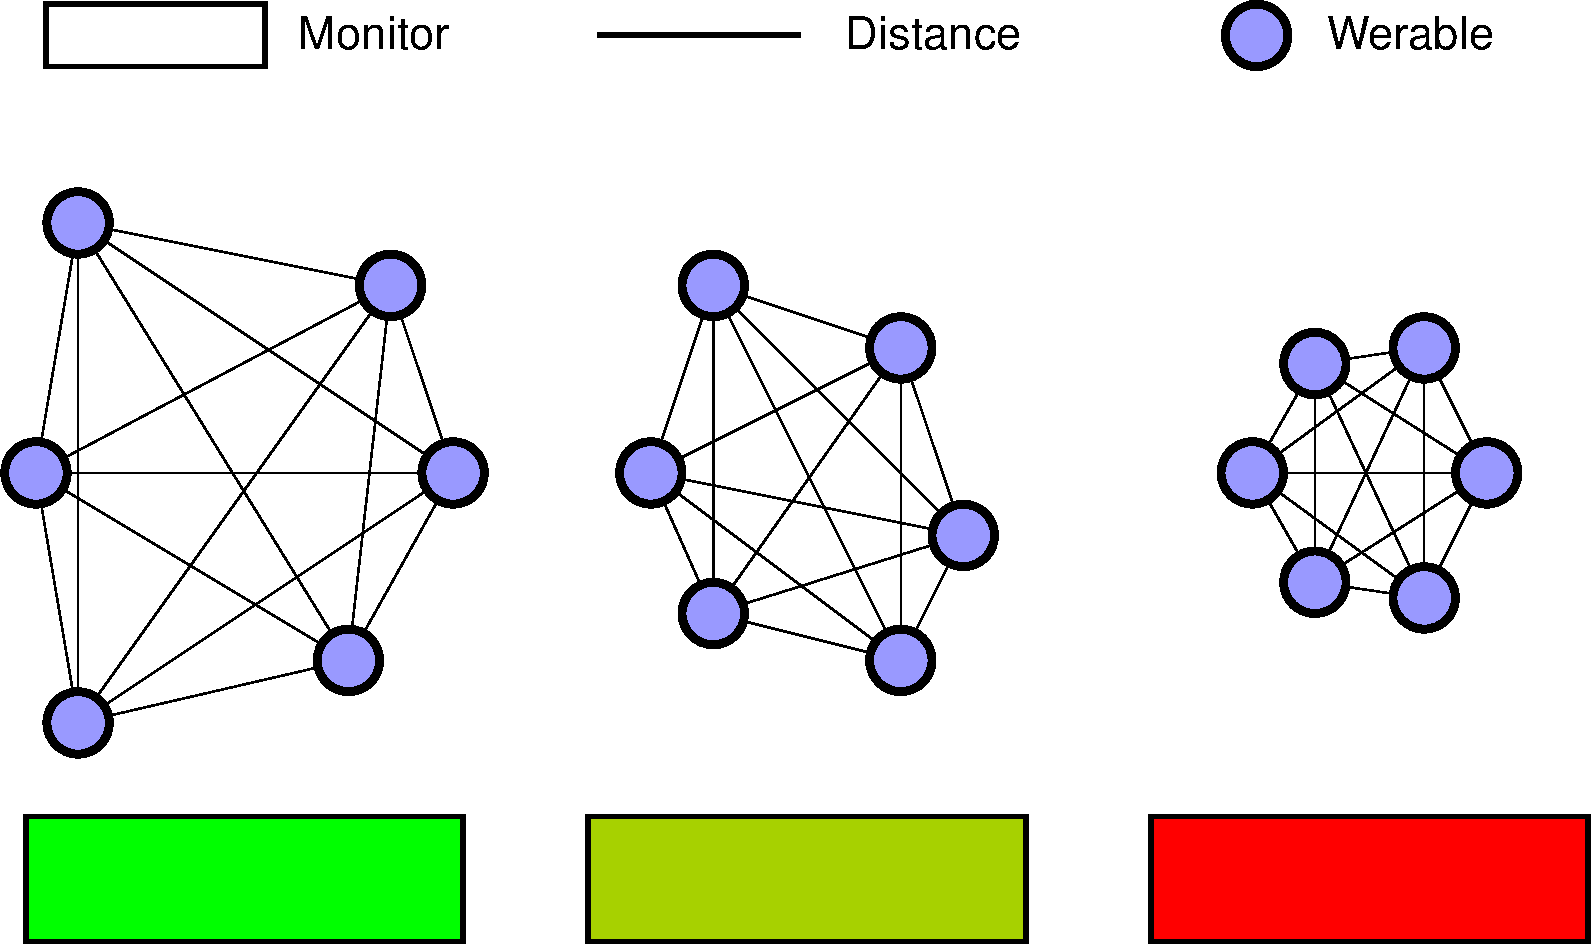
\includegraphics[width=\columnwidth]{figures/crow-laboratory-demo.drawio.pdf}
    \caption{
        Representation of the scenario described in \Cref{sec:small-scale-crowd-alert}.
        graph dots represent wearables,
        and arcs lenghts represent the distance between them.
        %
        The rectangle at the bottom represents the monitor.
        %
        The closer the wearables are, the higher is the alert level
        (reddish tones).
        %
        \meta{NICOLAS riduci lo spazio vuoto fra i tre casi, così da guadagnare spazio. La legenda potrebbe essere messa sotto o sopra per guadagnarne di ulteriore}
    }
    \label{fig:crowd-alert}
\end{figure}

The system is composed of two kinds of device: \emph{wearable} and \emph{alert}.
%
Wearables consist of the following pulverised components:
sensors ($\sigma^w$), perceiving other devices by their signal strenght;
behaviour ($\beta^w$), converting raw data from the sensor into messages for the alert system; and
communication ($\chi^w$) sending data to the alert system.
%
They do not need state nor actuators.
%
The alert consists of the following pulverized components:
$\beta^a$, computing the mean distance among devices;
$\kappa^a$ \meta{
    NICOLAS what does this do? write within this meta block
};
$\chi^a$, responsible for receiving the data from the wearable devices;
$\alpha^a$, enacting the alarm by showing a color on the screen.
%
It needs no sensors.

The infrastructure defined for this scenario is described as follow:

\begin{itemize}
    \item \emph{Smartphones} are the devices used by the people to detect the distance from the others;
    \item \emph{Local PC} is the device used to show the alarm in the laboratory;
    \item \emph{Server} is the device used run the crowd algorithm and the wearable logic. 
\end{itemize}

The initial deployment of the system starts with the $\beta_{werable}$ executed in the \emph{Server},
the $\sigma_{wearable}$ and $\chi_{werable}$ executed in the \emph{Smartphones},
and all the \emph{Laboratory} components are executed in the \emph{Local PC}.
%
Given the infrastracture defined above, we simulate also a condition where the \emph{Server} is overloaded and, via pulverization,
we want to lighteninig the load of the \emph{Server} by moving the $\beta_{werable}$ in the \emph{Smartphones}.
%
Formally, we can write the reconfiguration event as follow: $\beta^{werable}_{server} \xrightarrow{\mathcal{E}} \beta^{werable}_{smartphone}$
where $\mathcal{E}$ represents the reconfiguration event due to the high load in the \emph{Server}.

At the start of the system, each \emph{Werable} device, with the $\sigma$ component,
start to perceive the other devices in the laboratory using the RSSI signal from the Bluetooth.
%
The $\beta$ component, initially executed in the \emph{Server}, starts to compute the distances from the other devices
based on the received RSSI signal from the $\sigma$ component.
%
Once the distances are computed, the $\chi$ component sends the data to the
\emph{Laboratory} containing the dinstances perceived by the device.
%

Similarity, the \emph{Laboratory} device has all the components executed in the \emph{Local PC},
where the $\chi$ component receives the data from the \emph{Wearable},
the $\beta$ component computes the mean distance between the devices.
%
The $\kappa$ component persist in memory the updated devices grpah based on the distances retreived by the $\chi$ component.
and the $\alpha$ component show in the monitor the color based on the mean distance computed by the $\beta$ component.

As soon as the reconfiguration event is triggered, the $\beta$ component of the \emph{Werable} is moved from the \emph{Server} to the \emph{Smartphone}
lighteninig the server and preserving from one side the functional semantic of the system and from the other side maintain the system operational.
%
The reconfiguration of the system in entirely managed by the framework, which handle all the machinery and communication to move the component from
one host to another.
%
With this simple example we show how the pulverization framework can be used in practice to manage a system with different devices and an heterogeneous
infrastructure.
%
Moreover, we show how the pulverization framework can be used adapt the system to changing requirement without loosing the funcional semantic of the system
by describing the system in a declarative way.

\subsection{Large scale: urban event}

\cite{PianiniJOS2013}

\subsubsection{Free variables}

As follow are reported the free variables used in the evaluation:
\begin{itemize}
    \item let $n$ be the number of devices;
    \item let $t_d$ be the discharge time of the battery of the devices;
    \item let $B_l$ be the low battery threshold;
    \item let $B_h$ be the high battery threshold;
    \item let $EPI_{cloud}$ be the energy per instruction of the cloud;
    \item let $EPI_{ratio}$ be the ratio of the consumption of the cloud and the device;
\end{itemize}

\subsubsection{Metrics}

From the variables above are derived the following metrics:

\begin{itemize}
    \item let $\beta_{device}$ be the number of \emph{behaviour} executed in the device;
    \item let $\beta_{cloud}$ be the number of \emph{behaviour} executed in the cloud;
    \item let $C_{\%}$ be the average battery percentage of the devices;
    \item let $P_{devices}$ be the consumed power of the devices;
    \item let $P_{cloud}$ be the consumed power of the cloud;
    \item let $P_{total}$ be the total consumed power of the system;
    \item let $I_{cloud}$ be the number of server instances of the cloud;
    \item let $\$_{cloud}$ be the cost of the cloud;
\end{itemize}

\subsubsection{Results}

\begin{figure}[ht]
    \begin{minipage}{\columnwidth}
        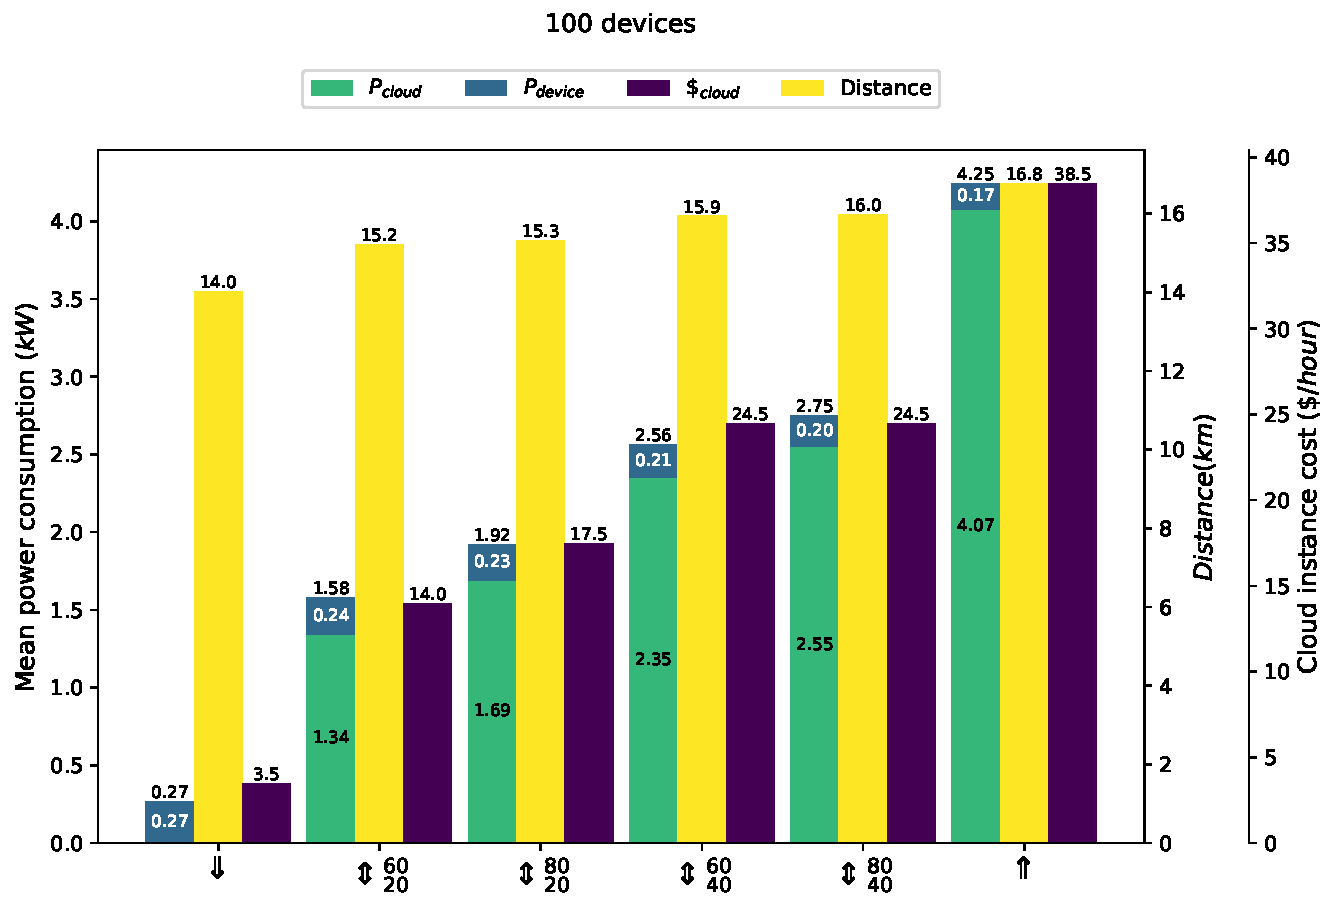
\includegraphics[width=\linewidth]{figures/cloud_cost-device_consumption-cloud_consumption-distance-device=100.0.pdf}
    \end{minipage}
    \caption{
        Results of the simulation with 100 devices.
        %
        The \emph{green} bar represents the mean power consumed by cloud;
        the \emph{blue} bar represents the mean power consumed by all the devices in the system;
        the \emph{yellow} bar represents the mean traveled distance by the people
        and the \emph{purple} bar represents the average cost per hour of the cloud.
        %
        The chart shows two ``static'' scenarios: \emph{device-only} (on the left) and \emph{cloud-only} (on the right).
        %
        All the intermediate scenarios are obtained by exploiting the reconfiguration capabilities of the pulverization framework,
        where different battery threshold are used to trigger the reconfiguration.
    }
    \label{fig:result-100-devices}
\end{figure}

\begin{figure}[ht]
    \begin{minipage}{\columnwidth}
        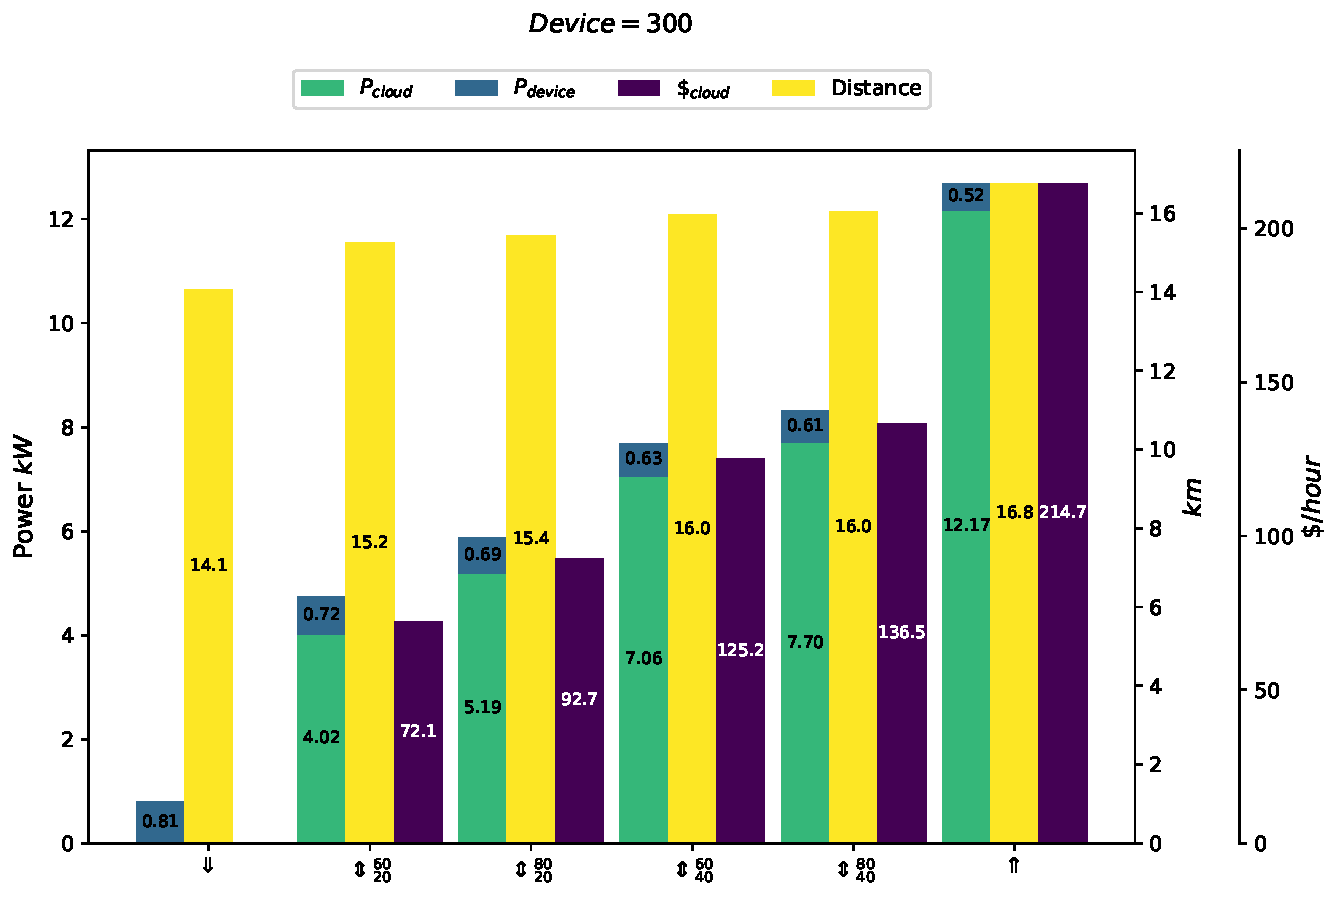
\includegraphics[width=\linewidth]{figures/cloud_cost-device_consumption-cloud_consumption-distance-device=300.0.pdf}
    \end{minipage}
    \caption{
        Results of the simulation with 300 devices.
        %
        The \emph{green} bar represents the mean power consumed by cloud;
        the \emph{blue} bar represents the mean power consumed by all the devices in the system;
        the \emph{yellow} bar represents the mean traveled distance by the people
        and the \emph{purple} bar represents the average cost per hour of the cloud.
        %
        The chart shows two ``static'' scenarios: \emph{device-only} (on the left) and \emph{cloud-only} (on the right).
        %
        All the intermediate scenarios are obtained by exploiting the reconfiguration capabilities of the pulverization framework,
        where different battery threshold are used to trigger the reconfiguration.
    }
    \label{fig:result-300-devices}
\end{figure}

\begin{figure}[ht]
    \begin{minipage}{\columnwidth}
        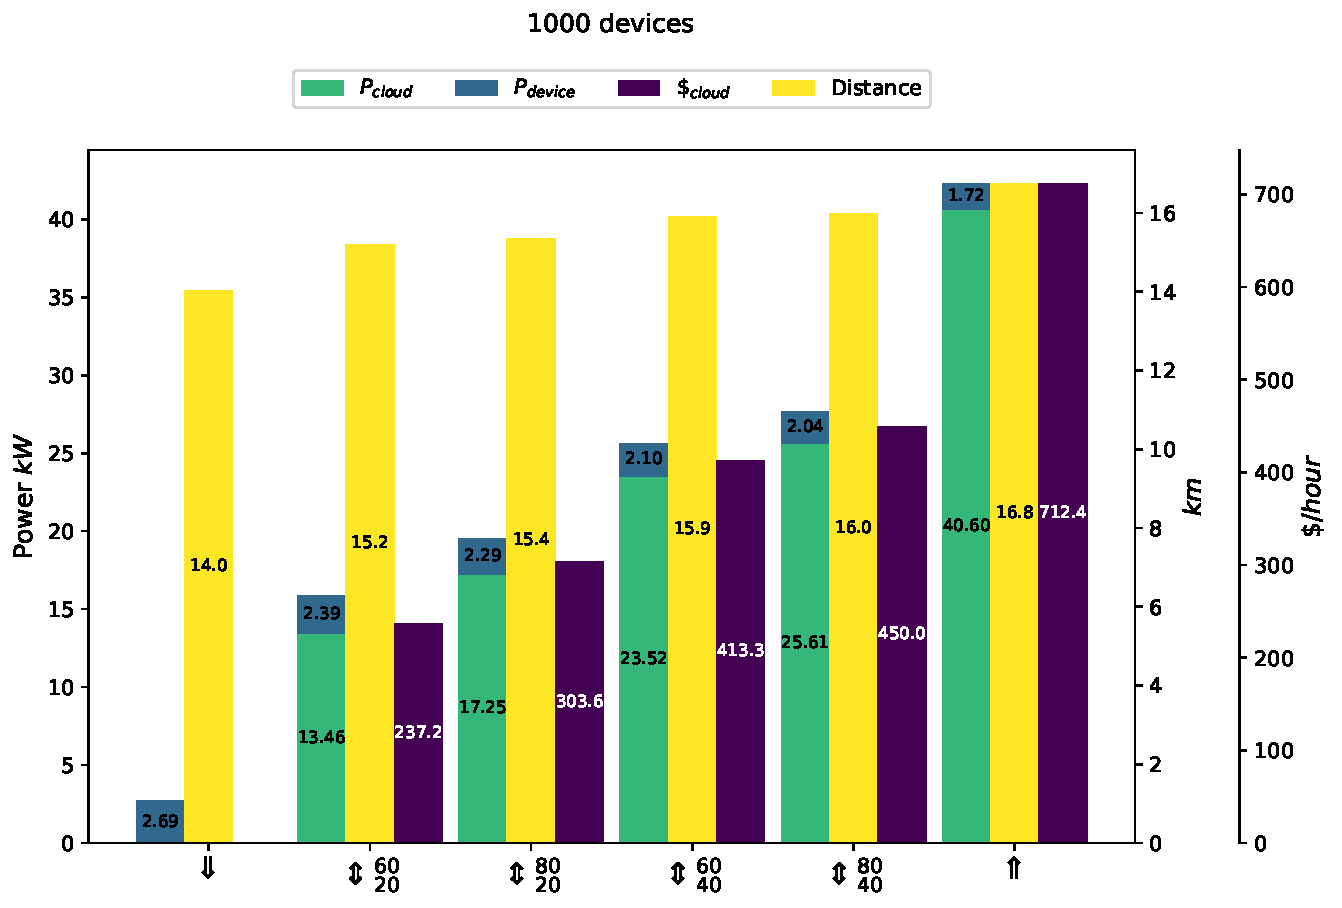
\includegraphics[width=\linewidth]{figures/cloud_cost-device_consumption-cloud_consumption-distance-device=1000.0.pdf}
    \end{minipage}
    \caption{
        Results of the simulation with 1000 devices.
        %
        The \emph{green} bar represents the mean power consumed by cloud;
        the \emph{blue} bar represents the mean power consumed by all the devices in the system;
        the \emph{yellow} bar represents the mean traveled distance by the people
        and the \emph{purple} bar represents the average cost per hour of the cloud.
        %
        The chart shows two ``static'' scenarios: \emph{device-only} (on the left) and \emph{cloud-only} (on the right).
        %
        All the intermediate scenarios are obtained by exploiting the reconfiguration capabilities of the pulverization framework,
        where different battery threshold are used to trigger the reconfiguration.
    }
    \label{fig:result-1000-devices}
\end{figure}




\section{Related Work}
\label{sec:rw}

%This work provides 
% \acp{dsl}
% for specifying 
% distributed systems (partitioned according to the 
% pulverisation model)
% and
% corresponding deployment plans,
% and a framework for executing
% deployment plans and reconfigurations.
%
Following the conceptual framework introduced in \Cref{sec:background:dep},
 in this section we cover related work about
 languages for 
 specifying distributed systems (\Cref{sec:rw:whatsw}),
 languages for specifying infrastructures and deployments (\Cref{sec:rw:depdesc}),
 and
 techniques for automatic deployment and reconfiguration (\Cref{sec:rw:autodep}).
 
 
 
\subsection{Application description languages: component-based software engineering and the pulverisation model}
\label{sec:rw:whatsw}
%
%% A first distinction revolves around whether 
%% the distributed software to be deployed 
%% is a monolith 
%% or is already broken into different components.
%
We consider a distributed application 
 as a graph of deployable units.
%
This partitioning may be 
 manually specified at development time
 (e.g., by explicitly defining and packaging different components)
 or automatically defined
 through \emph{application partitioning} approaches~\cite{DBLP:journals/jnca/LiuASGBQ15}. %exploiting the natural modularity of code (depending on the paradigm and language adopted).
 
In our approach, the application partitioning into components is manually specified through a \ac{dsl}.
%
Therefore, it can be framed in the context of \emph{component-based software engineering},
 with ~\cite{vale2016component-based-se} providing a comprehensive review.
%
The specification or design of distributed systems
 may leverage
 component models~\cite{DBLP:journals/tse/CrnkovicSVC11},
 architectural description languages~\cite{DBLP:journals/tse/MedvidovicT00},
 service-based compositions~\cite{DBLP:journals/csur/LemosDB16}, 
 or frameworks.
%

Specifically,
 this work builds on the \emph{pulverisation} component model~\cite{FI2020-pulverization,IEEE-IoTJ-pulverization-simulation},
 whereby a large-scale cyber-physical system
 is partitioned into a graph of devices
 where each device is split into five deployable components:
 (i) sensors interface, 
 (ii) actuators interface, 
 (iii) behaviour, 
 (iv) state, and 
 (v) communication component.
%
In~\cite{IEEE-IoTJ-pulverization-simulation},
 a methodology on top of the pulverisation model
 is proposed
 for generating and testing deployments through simulation.

Additionally,
 the approach of specifying in a single codebase 
 parts of the structure, behaviour, and/or interaction 
 for a whole distributed system
 is also related to \emph{macroprogramming}~\cite{Casadei2023macro}
 and, in particular, to \emph{multi-tier programming} paradigm~\cite{DBLP:journals/csur/WeisenburgerWS20},
 where the deployment units for different tiers (e.g., client and server tiers; or view, business logic, and data tiers) are obrained by compilation or interpretation of a single codebase.



\subsection{Infrastructure and deployment description languages}
\label{sec:rw:depdesc}

A \emph{deployment plan} is a configured mapping of a software system onto a deployment domain.
%
Given a deployable software system developed using the techniques of the previous subsection,
 what is needed now is a language to describe a deployment domain 
 and the deployment mapping.
%
Languages have been proposed 
 targetting specific kinds of deployment domains
 such as the smart grid (cf. the deployment specification language \emph{dspec} in the \emph{Resilient Information Architecture Platform for Smart Grids [RIAPS]} platform~\cite{DBLP:conf/coins/GhoshTKKL22})
 or the cloud (cf. the \emph{Cloud Application Modelling and Execution Language [CAMEL]} multi-\ac{dsl}~\cite{DBLP:journals/jcloudc/AchilleosKRKDOS19}).

In this work,
 we are especially interested deployments over large-scale cyber-physical systems and the edge-fog-cloud continuum.
%
The \emph{MultiScale Autonomic Deployment Language (MuScADeL)}~\cite{DBLP:conf/compsac/BoujbelRLTAL14/muscadel}
 is a \ac{dsl} that allows to express deployment properties of 
 componentised applications on multi-scale deployment domains, i.e., large and heterogeneous infrastructures considered under several viewpoints (device, geography, network, administrative domains, etc.).
%
In~\cite{DBLP:journals/sosym/SongDFSF22},
  a model-based deployment approach is proposed
  targetting so-called \emph{fleets}, i.e.,
  distributed and heterogeneous devices at the edge chaaracterised by different cyber-physical contexts (cf. resources, connectivity, etc.).
%
It is based on the \emph{Generation and Deployment
of Smart IoT Systems (GeneSIS)} modelling language, where a \texttt{DeploymentModel} consists of sets of \texttt{Resources} (e.g., \texttt{Component}s, specialised by \texttt{InfrastructureComponent}s and \texttt{SoftwareComponent}s) with associated \texttt{Property}s and \texttt{Link}s.

\subsection{Automatic/autonomic deployment and reconfiguration}
\label{sec:rw:autodep}
%
A comprehensive conceptual framework
 on automatic deployment of distributed systems
 is provided in a 2015 survey by Arcangeli et al. \cite{DBLP:journals/jss/ArcangeliBL15}.
%
A more recent survey by Coullon et al. focusses
 on formal techniques for verifying the correctness of reconfigurations
 in component-based distributed software systems~\cite{coullon2023swreconfig}.
%
Two formal models for specifying reconfigurable architectures are \emph{DR-BIP (Dynamically Reconfigurable - Behaviour Interaction Priority model)}~\cite{Ballouli18dr-bip}
and \emph{DReAM (Dynamically Reconfigurable Architectural Modelling)}~\cite{denicola2020dream-dynamic-reconfig-arch-modelling}.
%
Both are based on the same conceptual model: they 
 feature \emph{components} (capturing behaviour), \emph{connectors} (capturing interaction between components' \emph{ports}), 
\emph{maps} (logical topologies),
and \emph{deployments} (associating components to map locations),
overall organised in \emph{motifs} (dynamic architectural configurations),
to model and analyse dynamic architectures.
%
\meta{TODO: say something about our positioning wrt verification of reconfigurations}

In the \emph{osmotic computing} approach~\cite{DBLP:journals/computer/VillariFDRJR19},
 microservices (the solvent)
 can migrate across 
 the edge-cloud infrastructure (the solution),
 passing through layer boundaries (the semi-permeable membranes),
 in order to keep a balance in the desired properties (the solute).
%
The \emph{ASSL (Autonomic System Specification Language)}~\cite{DBLP:conf/birthday/VassevH97}
 supports the specification
 of autonomic elements,
 interaction protocols,
 and \emph{self-management policies} based on fluents (states), events, and actions.
%
%In \emph{ConfSolve}~\cite{DBLP:conf/saso/HewsonAG13},
% the language supports the specification of logical \emph{reconfiguration constraints}, which are then solved as a constraint satisfaction problem.
%
The \emph{AWaRE DSL (ADSL)}~\cite{DBLP:conf/aswec/ChhetriLUVKNR18/adsl} supports constraint-based self-management, leveraging managing agents. The language enables the specification of the domain model (in terms of components), the problem structure model (in terms of constraints), the agent architecture model (in terms of agents, roles, and their coordination), and the assignment model (in terms of management problem assignment strategies).
%
Similar, earlier approaches based on the specification of \emph{constraint-sets} include \emph{DELADAS}~\cite{Dearle2004deladas}
and \emph{ConfSolve}~\cite{DBLP:conf/saso/HewsonAG13}.
%
\emph{Ctrl-F}~\cite{DBLP:journals/jss/AlvaresRS17}
 is an architectural description language
 with constructs for specifying adaptive behaviour 
 and policies (constraints) for the reconfiguration of system components.
%
These approaches, however, typically suffer from scalability issues.

%%high-level constructs to describe adaptation in software components by means of behavioural programs, i.e., in terms of order and/or conditions under which reconfigurations take place; and policies, i.e., constraints that have to be enforced all along the execution. In other words, Ctrl-Fis a first-class language that is applicable to any Component-based application requiring self-adaptation with formal guarantees.
 
 

%\meta{
%MuScADeL (Multi-Scale Autonomic Deployment Language)~\cite{DBLP:conf/compsac/BoujbelRLTAL14/muscadel}
%
%ADSL (AWaRE DSL)~\cite{DBLP:conf/aswec/ChhetriLUVKNR18/adsl} % and see corresp RW: the most related DSLs are those in the area of automated deployment [17]. Such DSLs include Deladas [31], [32], ConfSolve [15], [33], j-ASD’s DSL [34] and MuScADeL [35], [36].DBLP:journals/jss/AlvaresRS17
%% [17]: J.-P. Arcangeli, R. Boujbel, and S. Leriche, "Automatic deployment of distributed software systems: Definitions and state of the art," Journal of Systems and Software, vol. 103, pp. 198–218, 2015
%%
%%%
%%%\subsection{Approaches to Deployment Independence}
%%%\label{s:rw:deployment-independence}
%%%
%%%\meta{TODO: add works on deployment independence, e.g., osmotic~\citep{DBLP:journals/computer/VillariFDRJR19}, BIP~\citep{lekidis2015bip-wsn,bastarrica2001optimization-techniques-deployment-components-bip}}
%%%
%%%We highlight a number of representatieve research efforts on deployment and automatic reconfiguration of systems.
%%%%
%%%%For instance, 
%%%\emph{Osmotic computing}~\cite{DBLP:journals/computer/VillariFDRJR19} is an approach to opportunistic deployment of microservices on the edge-fog-cloud platform.
%%%An osmotic platform aims to reach and maintain an ``osmotic equilibrium'' 
%%%between infrastructural and application requirements
%%%by automatically migrating microservices to deployment locations.
%%%
%%However, the approach mainly targets centrally orchestrated systems.
%%%
%%Other approaches leverage component-based, architectural descriptions to decouple application logic and deployment.
%%%
%%For instance, \emph{DR-BIP (Dynamically Reconfigurable - Behaviour Interaction Priority model)}~\cite{,Ballouli18dr-bip}
%%and \emph{DReAM (Dynamically Reconfigurable Architectural Modelling)}~\cite{denicola2020dream-dynamic-reconfig-arch-modelling}
%%use \emph{components} (capturing behaviour), \emph{connectors} (capturing interaction between components' \emph{ports}), 
%%\emph{maps} (logical topologies),
%%and \emph{deployments} (associating components to map locations),
%%overall organised in \emph{motifs} (dynamic architectural configurations),
%%to model and analyse dynamic architectures.
%%%
%%
%%These approaches have some similarity with the approach presented in this paper, but they are arguably more complex and our  
%%%than the one introduced in this paper,
%% %, though also fostering an exogenous, declarative (logics-based) modelling approach.
%%approach explicitly addresses self-organising CPS.
%%%
%%%
%%%By constrast, our approach explicitly addresses self-organising CPS.
%%%
%%%A more in-depth, formal comparison is left as future work.
%}

\section{Conclusion and future work}\label{sec:conclusion}

openness

more platforms

global policies

\bibliographystyle{IEEEtran}
\bibliography{bibliography}

%\vspace{12pt}
%\color{red}
%IEEE conference templates contain guidance text for composing and formatting conference papers. Please ensure that all template text is removed from your conference paper prior to submission to the conference. Failure to remove the template text from your paper may result in your paper not being published.

\end{document}
